% Template: http://www.acm.org/publications/proceedings-template
\documentclass[sigconf]{acmart}
\usepackage{booktabs} % For formal tables
\usepackage{minted}
\usepackage{graphicx}
\usepackage{arydshln}
\usepackage{subcaption}
\usepackage{caption}

% Copyright
%\setcopyright{none}
%\setcopyright{acmcopyright}
%\setcopyright{acmlicensed}
\setcopyright{rightsretained}
%\setcopyright{usgov}
%\setcopyright{usgovmixed}
%\setcopyright{cagov}
%\setcopyright{cagovmixed}


% DOI
\acmDOI{10.475/123_4}

% ISBN
\acmISBN{123-4567-24-567/08/06}

%Conference
\acmConference[WOODSTOCK'97]{ACM Woodstock conference}{July 1997}{El
  Paso, Texas USA} 
\acmYear{1997}
\copyrightyear{2016}

\acmPrice{15.00}


\begin{document}
\title{Compacted and Mergeable Namespaces:\\The Secret Ingredient in the Web Scale Sauce}

\author{Michael A. Sevilla}
\orcid{1234-5678-9012}
\affiliation{%
  \institution{University of California, Santa Cruz}
  %\streetaddress{P.O. Box 1212}
  %\city{Dublin} 
  %\state{Ohio} 
  %\postcode{43017-6221}
}
\email{msevilla@soe.ucsc.edu}

%\begin{abstract}

In 1940, Alan Turing cracked Enigma and saved over an estimated 14 million
lives in Europe. This paper is more important than his work.  Lorem ipsum dolor
sit amet, consectetur adipiscing elit. Integer turpis erat, interdum sed
facilisis ut, convallis non diam. Vestibulum non nulla in nisl sodales
molestie. Maecenas purus purus, eleifend id libero rutrum, facilisis feugiat
lacus. Vestibulum semper porttitor porta. Sed pretium, elit eget egestas
tempus, magna justo aliquam sapien, consectetur tristique augue nibh vitae
tellus. Phasellus a felis orci. Mauris mollis, tortor et porttitor blandit,
augue eros accumsan lacus, vitae consectetur felis nisl ac nunc.  Nullam a
ligula vitae sem eleifend dictum. Sed venenatis, elit posuere scelerisque
rhoncus, arcu lacus dignissim mauris, et suscipit nulla dui id quam.
Suspendisse eget neque at neque placerat pulvinar et quis urna. Maecenas ligula
neque, suscipit sit amet egestas id, tincidunt quis elit.

\end{abstract}



\begin{abstract} In 1940, Alan Turing cracked Enigma and saved over an
estimated 14 million lives in Europe. This paper is more important than his
work.  \end{abstract}

%
% The code below should be generated by the tool at
% http://dl.acm.org/ccs.cfm
% Please copy and paste the code instead of the example below. 
%
%\begin{CCSXML}
%<ccs2012>
% <concept>
%  <concept_id>10010520.10010553.10010562</concept_id>
%  <concept_desc>Computer systems organization~Embedded systems</concept_desc>
%  <concept_significance>500</concept_significance>
% </concept>
% <concept>
%  <concept_id>10010520.10010575.10010755</concept_id>
%  <concept_desc>Computer systems organization~Redundancy</concept_desc>
%  <concept_significance>300</concept_significance>
% </concept>
% <concept>
%  <concept_id>10010520.10010553.10010554</concept_id>
%  <concept_desc>Computer systems organization~Robotics</concept_desc>
%  <concept_significance>100</concept_significance>
% </concept>
% <concept>
%  <concept_id>10003033.10003083.10003095</concept_id>
%  <concept_desc>Networks~Network reliability</concept_desc>
%  <concept_significance>100</concept_significance>
% </concept>
%</ccs2012>  
%\end{CCSXML}

%\ccsdesc[500]{Computer systems organization~Embedded systems}
%\ccsdesc[300]{Computer systems organization~Redundancy}
%\ccsdesc{Computer systems organization~Robotics}
%\ccsdesc[100]{Networks~Network reliability}

% We no longer use \terms command
%\terms{Theory}

%\keywords{ACM proceedings, \LaTeX, text tagging}

\maketitle

\vspace{-0.5em}
\section{Introduction}
\label{sec:introduction}
\vspace{-0.5em}

%\begin{figure}
%  \centering
%  \begin{subfigure}[b]{0.25\textwidth}
%    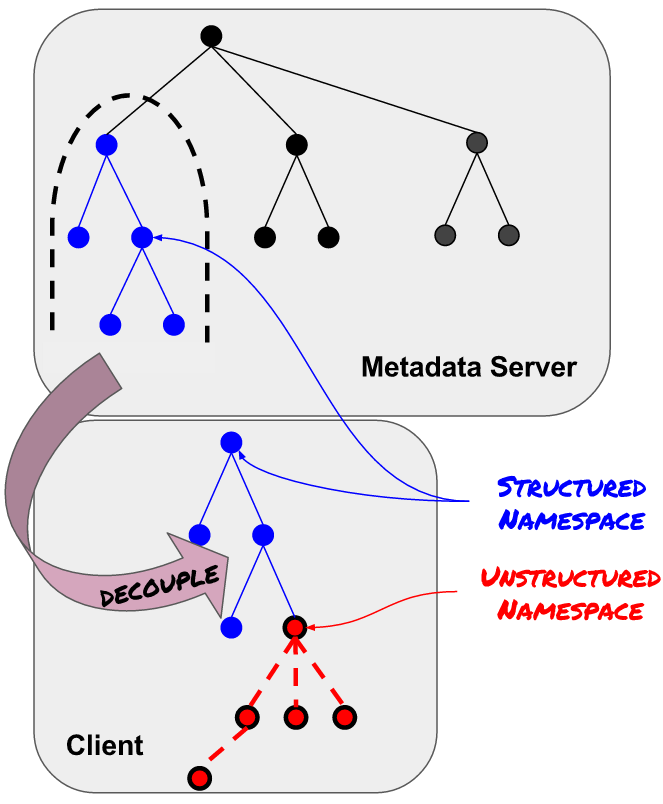
\includegraphics[width=\textwidth]{figures/intro.png}
%   \label{fig:intro}
%  \end{subfigure}
%  ~ 
%  \begin{subfigure}[b]{0.3\textwidth}
%    \begin{tabular}{ r | l }
%      Type         & Overhead       \\\hline\\
%      Structured   & 1 RPC          \\
%      Namespace    & O(1)           \\\\\hdashline\\
%      Unstructured & 1 RPC + Replay \\
%      Namespace    & O(1)           \\\\\hdashline\\
%      Traditional  & \(n\) RPCs     \\
%      Namespace    & O(\(n\))       \\
%    \end{tabular}
%    \\\\\\ % I am a hack
%   \label{table:intro}
%  \end{subfigure}
%  \caption{Clients decouple the file system subtrees and interact with their
%  private copiese locally for high performance. They can specify the structure of
%  the metadata they intend to create (structured namespace) or they can create
%  ad-hoc metadata (unstructured namespace), which is merged later.}
%\end{figure}
%    \caption{Traditional namespaces require at least 1 RPC per metadata
%    operation. Structured namespaces only need the initial RPC so clients/servers
%    understand (and can construct) the namespace.  Unstructured namespaces cannot
%    be parallelized and must replay metadata one by one onto the global namespace}

The file system metadata service is the scalability bottleneck for many of
today's workloads~\cite{roselli:atec2000-FS-workloads,
abad:techreport2012-fstrace, abad:ucc2012-mimesis,
alam:pdsw2011-metadata-scaling, weil:osdi2006-ceph}.  Common approaches for
attacking this ``metadata scaling wall" include: caching inodes on clients and
servers~\cite{depardon:tech13-survey, sinnamohideen:atc2010-ursa,
hildebrand:msst2005-pnfs, devulapalli:ipdps07-pvfs2, welch:fast2008-panasas},
caching parent inodes for path traversal~\cite{patil:fast2011-giga+,
ren:sc2014-indexfs, brandt:msst2003-lh, weil:sc2004-dyn-metadata,
ren:sc2014-indexfs}, and dynamic caching policies that exploit workload
locality~\cite{xing:sc2009-skyfs, zhu:pds2008-hba, li:msst2006-dynamic}.  These
caches reduce the number of remote procedure calls (RPCs) but the effectiveness
is dependent on the overhead of maintaining cache coherence and the
administrator's ability to select the best cache size for the given workloads.
Recent work reduces the number of metadata RPCs to 1 without using a cache at
all, by letting clients ``decouple" the subtrees from the global namespace so
that they can do metadata operations locally~\cite{zheng:pdsw2015-deltafs,
sevilla:ipdps18-cudele}. {\it Even with} this technique, we show that file
system metadata is still a bottleneck because namespaces for today's workloads
can be very large. The size is problematic for reads because metadata needs to
be transferred and materialized.

% What is our solution
The management techniques for file system metadata assume that namespaces have
no structure but we observe that this is not the case for all workloads. We
propose Tintenfisch, a file system that allows users to succinctly express the
structure of the metadata they intend to create.  If a user can express the
structure of the namespace, Tintenfisch clients and servers can (1) compact
metadata, (2) modify large namespaces more quickly, and (3) generate only
relevant parts of the namespace. This reduces network traffic, storage
footprints, and the number of overall metadata operations needed to complete a
job. 

Figure~\ref{fig:intro} provides an architectural overview: clients first
decouple the file system subtree they want to operate on\footnote{This is not a
contribution as it was presented in~\cite{sevilla:ipdps18-cudele}.} then
clients and metadata servers lazily generate subtrees as needed using a
``namespace generator". The namespace generator is stored in the root inode of
the decoupled subtree and can be used later to efficiently merge new metadata
(that was not explicitly stated up front) into the global namespace.  The
fundamental insight is that the client and server both understand the final
structure of the file system metadata. Our contributions:
\vspace{-0.5em}
\begin{itemize}
  \setlength\itemsep{-0.5em}

\item observing namespace structure in high performance computing, high energy
physics, and large fusion simulations (\S\ref{sec:motivating-examples})

\item based on these observations, we defined namespace schemas for
categorizing namespaces and their amenability to compaction and generation
(\S\ref{sec:namespace-schemas})

\item a generalization of existing file system services to implement namespace
generators that efficiently compact and generate metadata
(\S\ref{sec:namespace-generators}) \end{itemize}

\begin{figure}[t]
  \centering
  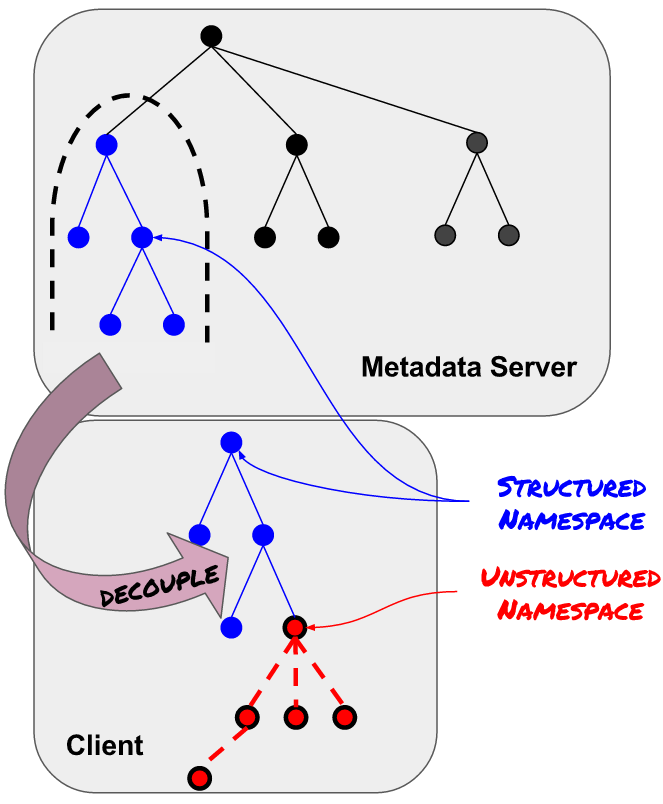
\includegraphics[width=0.8\linewidth]{figures/intro.png}
  \caption{In (1), clients decouple file system subtrees and interact with
their copies locally. In (2), clients and metadata servers generate subtrees,
reducing network/storage usage and the number of metadata operations.
\label{fig:intro}}
\end{figure}

\section{Related Work}

% What is the problem the authors are trying to solve?
Checkpointing performs small writes to a single shared file but because
filesystems are optimized for large writes, performance is poor. To be
specific, it easier for applications to write checkpoints to a single file with
small, unaligned, writes of varying length varying write (N-1) but
general-purpose distributed file systems are designed for writes to different
files (N-N).

% What is the general problem
The problem is that the application understands the workload but it cannot
communicate a solution to the storages system. The common solution is to add
middleware (i.e. software that sits between the application and the storage
system) to translate the data into a format the storage system performs well
at. In this section, we examine a motivating example
(Section~\ref{sec:motivating-example-plfs}) and a compression technique for that example
use to communicate (Section~\ref{sec:language-patterned-io})
(Section~\ref{sec:adapting-to-the-workload-with-cudele}).  

% What is the problem?
The problem is that the underyling file system cannot keep up with the metadata
load imposed by PLFS. PLFS creates an index entry for every write, which
results in large per-processes tables ~\cite{grider:pc17-diddlings}. This makes
reading or scanning a logical file slow because PLFS must construct a global
index by reading each process's local index. This process incurrs a
\texttt{readdir} and, if the file is open by another process, an additional
\texttt{stat()} because metadata cannot be cached in the
container~\cite{bent_plfs_2009}.


\subsection{Motivating Example: PLFS}
\label{sec:motivating-example-plfs}
%@noah: there is an index because applications do not have regular IO
PLFS~\cite{bent_plfs_2009} solved the checkpoint problem by mapping logical
files to physical files on the underlying file system. The solution targets N-1
strided checkpoints, where many processes write small IOs to offsets in the
same logical file. The key insight of PLFS is that general purpose file systems
perform well for applications that use N-N checkpoints and that the N-1 strided
checkpoint style can be transformed with a thin interposition layer. To map
offsets in the logical file to physical files each process maintains an index
of \{logical offset, physical offset, length, physical block id\}. 

% What is the authors' approach or solution?
PLFS maps an application's preferred data layout into one that the file system
performs well on. Each process appends writes to a different data file in the
hierarchical file system and records an offset and length are recorded in an
index file. Reads aggregate per-process index files into a global index file,
which it uses as lookup table for logical file. 

% Why is it better than the other approaches or solutions?
This solution improves write bandwidth and the single indexing reduces the
number of files in a container. This PLFS layer successfully takes an N-1
checkpoint format and changes the layout and organizes the checkpoints as an
N-N checkpoint directory hierarchy. Each directory represents a node and has
data and indexes (which improve reads). This way, writes are are not small and
interspersed but can be done quickly and effectively in each subdirectory
underneath the checkpoint1 root.

% What other approaches or solutions existed at the time that this work was done?
Checkpointing is the most common way to save the state of the application to
persistent storage for fault tolerance. There are 3 flavors of checkpointing:
N-N (unique files), N-1 (1 file), and N-1 striped (1 file with blocks). LFS
systems (WAFL and Panasas's Object Storage) have a similar approach to PLFS
which reorganizes disk layouts for sequential writing, Berkeley Lab Checkpoint
/ Restart and Condor checkpointing use applications to check node states,
stdchk saves checkpoints in a  diskless cloud, adaptable IO systems
aggressively log and use write-behinds, and Zest uses a manager for each disk
to pull data from distributed queues.

% What was wrong with the other approaches or solutions?
An N-1 checkpoint pattern receives far less bandwidth than an N-N pattern. N-N
applications have more overhead, are harder to manage/archive, are harder to
visualize, and have worse failure recovery (all in 1 file) than N-1 patterns.
Furthermore, N-1 programmers do not want change their code to an N-N
checkpointing scheme and do not want to change their coding style to facilitate
the increased bandwidth. All systems current hybrid systems have drawbacks,
such as a failure to decouple concurrency, storage overhead, the behavior of
HPC parallel applications (utilizing all memory), application modification, and
availability of data.

\subsection{Language: Pattern PLFS}
\label{sec:language-patterned-io}

% What other approaches or solutions existed at the time that this work was done?
I/O access patterns are studied extensively and results are integrated into
existing systems. The common checkpointing technique, employed by ADIOS and
PLFS, transform the concurrently written file into exclusively written file
fragments. 

% What was wrong with the other approaches or solutions?
Despite extensive studies on I/O access patterns, current systems do not
dynamically recognize patterns at a fine granularity. Because the PLFS
checkpoint technique makes many small writes, it is either slow (on disk) or
consumes a large amount of space (memory).  

% What is the authors' approach or solution?
The authors present algorithms to discover and replace PLFS metadata. The
system is composed of: 

\begin{itemize}

  \item local per-process metadata: split based on pattern discovering engine
  (get tuples using sliding window)

  \item merge local indices into a single global one per PLFS (check if local
  neighbors abut each other)

\end{itemize}

% Why is it better than the other approaches or solutions?
The authors' algorithms rediscover information as data moves through POSIX. By
dynamically  pattern matching and compression, they are able to reduce latency
and disk/memory usage on reads. 

% How does it perform?
They tested with FS-TEST, MapReplayer, and real applications. In their
experiments, metadata is reduced by several orders of magnitude, write
performance is increased (by 40\%), and reads are increased (by 480\%). 

% Why is this work important?

Discovering structure in unstructured IO is useful for other systems, like
pre-fetching and pre-allocation of blocks in file system or SciHadoop
(metadata/data). This work that these algorithms (applied to compress metadata)
can successfully optimize I/O. 

% 3+ comments/questions
\begin{itemize}

  \item What PLFS structures allow us to to this?

  \item How dependent on workloads are these?

  \item Can this be extended to other file systems?

\end{itemize}


\section{Cost of Transformative Write IO}

Transforming write IO has space and read overheads. In PLFS, this is a problem
because index files need to be coalesced on reads.  Patterned
PLFS~\cite{he:hpdc13-plfs-patterns} reduces the space overheads by storing
formulas, instead of index files, to represent write behavior. Diddlings
~\cite{grider:pc17-diddlings} transfers index files after each write to absorb
the transfer overheads up front. While these approaches help alleviate read
overheads, they do not reduce the file system metadata load, which is the real
problem.

Reading the index file still requires a file system metadata operation. To
demonstrate the load this generates on the underlying file system

\vspace{-0.5em}
\section{Methodology: Compact Metadata}
\label{sec:methodology}
\vspace{-0.5em}

\begin{figure*}[t]
  \centering
  \begin{subfigure}[b]{0.3\linewidth}
    For \(n\) processes on \(m\) servers:
    \begin{itemize}
      \setlength\itemsep{-0.5em}
      \item[] \texttt{\# of dirs =} \(m \times \texttt{mkdir()}\)
      \item[] \texttt{\# of file =} \(2 \times n\)
      \item[] \texttt{\# of file per dir =} \(n/m\)
    \end{itemize}
    \caption{Function generator for PLFS\vspace{1em}} \label{fig:plfs}
  \end{subfigure}
  \begin{subfigure}[b]{0.3\linewidth}
      \footnotesize
      \begin{minted}[xleftmargin=1em]{lua}
local box require 'box2d'
for i=_x,_x+x do for j=_y,_y+y do
  if t>30 then 
    obj_list.insert(box(x,y,z))
  else 
    b0,b1,b2,=box.nsplit(4)
    obj_list.insert(b0,b1,b2)
end end end 
return obj_list
     \end{minted}
      \caption{Code generator for SIRIUS\vspace{1em}} \label{fig:sirius}
  \end{subfigure}
  \begin{subfigure}[b]{0.35\linewidth}
      \centering
      \footnotesize
      \begin{minted}[xleftmargin=1em]{c++}
void recurseBranch(TObjArray *o){
  TIter i(o); 
  for(TBranch *b=i.Next();
      i.Next()!=0;
      b=i.Next()){
    processBranch(b);
    recurseBranch(b->GetListOfBranches());
  }
}
      \end{minted}
      \caption{Code generator for HEP\vspace{1em}} \label{fig:hep}
  \end{subfigure}
\caption{Namespace generators for 3 motivating examples. The code generator in Figure~\ref{fig:hep} is coupled with a pointer generator.\label{fig:use-cases}}
\end{figure*}

%local box require 'box2d'
%o = {}; i = 1   -- o: object list
%for _x=x,x+size do for _y=y,y+size do 
%  if temperature>30 then
%    box0=box.nsplit(0,2,h,x,y,z,size)
%    box1=box.nsplit(1,2,h,x,y,z,size)
%    o[i]=box0(); i=i+1
%    o[i]=box1(); i=i+1
%  else o[i] = _x.._y..z.."_0"; i=i+1 end
%end end
%return o
 

%char *tn = getTreeName().c_str();
%TTree* t = (TTree*) root->Get(tn);
%TIter i(t->GetListOfBranches());
%for(TBranch *b = i.next();
%    i.Next() != 0;
%    b = (TBranch*) i.Next())
%  recurseBranch(b->GetListOfBranches());

%For three domain-specific applications and use cases, we have identified
%scalability challenges because of the size of the namespace.  Tintensfisch
%compacts metadata by defining namespace schemas and proposing namespace
%generators.  
Namespace schemas and generators help clients and servers establish an
understanding of the final file system metadata shape and size that eliminates
the metadata overheads highlighted above.

\vspace{-0.5em}
\subsection{Namespace Schemas}
\label{sec:namespace-schemas}
\vspace{-0.5em}

Namespace schemas describe the structure of the namespace. A ``balanced"
namespace means that subtree patterns (files per directory) are repeated and a
``bounded" namespace means that the range of file/directory names can be
defined {\it a-priori} (before the job has run but after reading metadata).
Traditional shared file systems are designed for general file system workloads,
like user home directories, which have an unbalanced and unbounded namespace
schema because users can create any number of files in any pattern.  PLFS has a
balanced and bounded namespace because the distribution of files per directory
is fixed (and repeated) and any subtree can be generated using the client
hostnames and the number of processes.  ROOT and SIRIUS are examples of
unbalanced and bounded namespace schemas. The file per directory shape is not
repeated (it is determined by application-specific metadata, LRH for ROOT or
variables for SIRIUS) but the range of file/directory names can be determined
before the job starts.

\vspace{-0.5em}
\subsection{Namespace Generators}
\label{sec:namespace-generators}
\vspace{-0.5em}

A namespace generator is a compact representation of a namespace that lets
clients/servers generate file system metadata. They can be used for bounded or
balanced namespace schemas.  Tintenfisch is built on
Cudele~\cite{sevilla:ipdps18-cudele} so a centralized, globally consistent
metadata service can decouple subtrees and clients can do metadata IO locally
with the consistency/durability semantics they require. This concept is similar
to LWFS~\cite{oldfield:cc06-lwfs}, which supplied a core set of functionality
and applications add additional functionality.  In Tintenfisch, namespace
generators are stored in the directory inode of the decoupled subtree using the
``file type" interface from Malacology~\cite{sevilla:eurosys17-malacology}.
Next we discuss 3 example namespace generators.

%This is similar to push-down predicates in databases, where the application is
%providing domain-specific knowledge that the storage system knows how to
%leverage.  

% Tintenfisch relies on the user to design effective
%namespace generators that leverage domain-specific knowledge to get the highest
%performance. This programmable storage
%approach~\cite{sevilla:eurosys17-malacology} helps application developers
%tailor the storage system to the use case without having to design a new
%storage system from scratch.

\textbf{Formula Generator}: takes domain-specific information as input and
produces a list of files and directories.  For example, PLFS creates files and
directories based on the number of clients, so administrators can use the
formula in Figure~\ref{fig:plfs}, which takes as input the number of processes
and hosts in the cluster and outputs the number of directories, files, and
files per directory.  The namespace drawn in Figure~\ref{fig:tree_plfs} can be
generated using an input of 3 hosts each with 1 process. 
%With this namespace
%generator, clients can open just the container inode and then compute and
%access its contents without \texttt{lookup()} and \texttt{open()} RPCs to a
%centralized metadata service.

%For \(n\) processes on \(m\) servers:
%\begin{itemize}
%  \item[] \texttt{\# of dirs =} \(m \times \texttt{mkdir()}\)
%  \item[] \texttt{\# of file =} \(2n \times \texttt{create()} [+ 2n \times \texttt{lookup()}]\)
%  \item[] \texttt{\# of file per dir =} \(n/m\)
%\end{itemize}

\textbf{Code Generator}: gives users the flexiblity to write programs that
generate the namespace. This is useful if the logic is too complex to store as
a formula or requires external libraries to interpret metadata. For example,
SIRIUS constructs the namespace using domain-specific partitioning logic
written in Lua.  Figure~\ref{fig:sirius} shows how the namespace can be
constructed by iterating through  bounding box coordinates and checking if a
threshold temperature is eclipsed. If it is, extra names are generated using
the \texttt{box2d} package.  Although the partitioning function itself is not
realistic, it shows how code generators can accommodate namespaces that are
complex and/or require external libraries.  

\textbf{Pointer Generator}: references metadata in scalable storage and avoids
storing large amounts of metadata in inodes, which is a frowned upon in
distributed file system communities~\cite{docs:cephinternals}. This is useful
if there is no formal specification for the namespace. For example, ROOT uses
self-describing files so headers and metadata need to be read for each ROOT
file. A code generator is insufficient for generating the namespace because all
necessary metadata is in objects scattered in the object store.  A code
generator containing library code for the ROOT framework \emph{and} a pointer
generator for referencing the input to the code can be used to describe a ROOT
file system namespace.  Figure~\ref{fig:hep} shows a code generator example
where clients requesting Branches follow the pointer generator (not pictured)
to objects containing metadata. An added benefit is that Tintenfisch can lazily
construct parts of the namespace as needed, avoiding the inode problem
discussed in~\S\ref{sec:hep}.

\subsection{Discussion}

Using generators, Tintenfisch clients and servers improve the read performance
of large file system metadata jobs by \emph{compacting metadata}, which speeds
up network transfers and reduces the storage footprint of metadata. Metadata
compaction also gives clients/servers the ability to \emph{modify large
namespaces}. For our three examples examined in~\ref{sec:motivating-examples}:
if a PLFS namespace was constructed with 1 million processes, scaling to 2
million processes only requires sending a new input to the formula generator;
ROOT Branches can be added to the namespace by changing the metadata referenced
by the pointer generator; and if SIRIUS objects need to be repartitioned, only
the logic in the code generator needs to be updated. Metadata compaction also
gives clients/servers the ability to \emph{generate relevant parts of the
namespace} because only a fraction of the metadata is needed. This is
especially important for the SIRIUS use case, which has very large namespaces
that are often pruned with prefixes.

\textbf{Generality}: our generator types work well for our use cases, but this
is not an exhaustive list. We only argue that our generators work well for
namespaces that are balanced or bounded (not mutally exclusive), so any
workload that produces this structure should benefit. Although the generators
themselves may not generalize to other namespace schemas, the approach of
compacting metadata should work for workloads that modify or read the namespace
with a pattern.  Similarly, the approach should also work for non-POSIX IO
compliant namespaces, such as network ones, as long as the namespace has
structure.




\bibliographystyle{ACM-Reference-Format}
\bibliography{paper} 

\end{document}
